\documentclass[12pt]{article}

\usepackage[a4paper,width=160mm,top=20mm,bottom=20mm,bindingoffset=6mm]{geometry}
\usepackage[utf8]{inputenc}
\usepackage[italian]{babel}
\usepackage[OT1]{fontenc}
\usepackage{graphicx}
\usepackage{float}
\usepackage{fancyhdr}
\usepackage{xcolor}
\usepackage{mathtools}
\usepackage{amsmath}
\usepackage{amssymb}
\usepackage{tikz}
\usepackage{imakeidx}
\usepackage{textcomp}
\usepackage{pifont}
\usepackage{polynom}
\usepackage{algorithm}
\usepackage{algpseudocode}
\usepackage{mathtools}
\usepackage[colorlinks=true,linkcolor=black,anchorcolor=black,citecolor=black,filecolor=black,menucolor=black,runcolor=black,urlcolor=black]{hyperref}
\usepackage{cancel}
\usepackage{pgfplots}
\usepackage{caption}
\usepackage{tabularx}
\usepackage{comment}
\usepackage{float}
\usepackage{bm}



\begin{document}
\bibliographystyle{plain}
    \pagestyle{fancy}
    \everymath{\displaystyle}
    \sffamily
    \begin{figure}
        \centering
        
\includegraphics[scale=0.1]{images/uniba-logo.png}
        \caption*{Università degli Studi di Bari Aldo Moro}
    \end{figure}
    
    \title{Relazione tecnica Sustainability of RecSys}
    \author{Emanuele Fontana}
    \date{Tirocinio tesi triennale in Informatica\\Anno accademico 2023/2024}
    \maketitle
    \tableofcontents\newpage
    \section{Design esperimenti}



\noindent Il lavoro svolto consiste nel: 
\begin{itemize}
    \item valutare e prevedere l'impatto ambientale di un sistema di raccomandazione (RecSys) in base alla sua sostenibilità
    \item cercare una soluzione per ridurre l'impatto ambientale di un RecSys senza però perdere di performance in modo significativo.
\end{itemize}

\noindent Nella prima parte dunque sono stati effettuati ulteriori esperimenti per valutare l'impatto ambientale di diversi modelli di raccomandazione su diversi dataset. Questi dati sono stati utilizzati per addestrare un modello di regressione che permette di prevedere le emissioni prodotte da un modello di raccomandazione in base a diversi parametri.


\noindent Nella seconda parte, invece, ci si è concentrati su come ridurre l'impatto ambientale di un RecSys senza però perdere di performance. In particolare, si è cercato di capire se fosse possibile ridurre le emissioni prodotte da un modello di raccomandazione senza però perdere di performance in modo significativo.



\noindent Per quanto riguarda la valutazione, mediante la libreria CodeCarbon\footnote{\href{http://codecarbon.io}{CodeCarbon}}{} è stato possibile misurare le emissioni prodotte dalla macchina durante l'addestramento con parametri di default per un dato modello dato un dataset. 
In questo ambito  Spillo et al.\cite{spillo2023towards} mostrano come spesso algoritmi più semplici riescono ad avere delle performance molto simili a modelli più complessi, ma con un impatto ambientale decisamente minore.

\section{Situazione Attuale}


\subsection{Introduzione}

\noindent Per quanto riguarda la previsione questo prima parte del documento si propone di presentare lo stato attuale del lavoro svolto in questo ambito.

\begin{figure}[H]
    \centering
    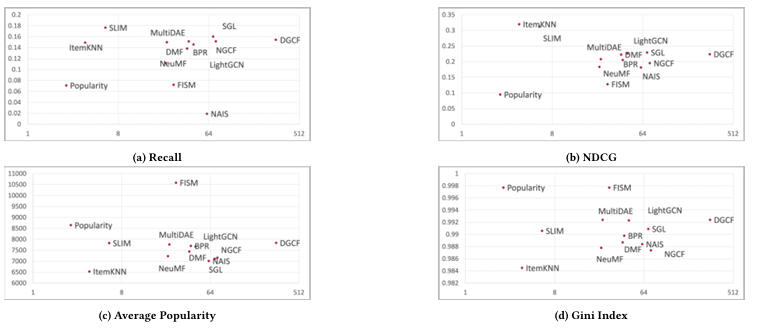
\includegraphics[scale=0.75]{images/risultati-valutazione.png}
    \caption{Trade-off tra emissioni e performance con dataset Mind}


\end{figure}



\begin{figure}[H]
    \centering
    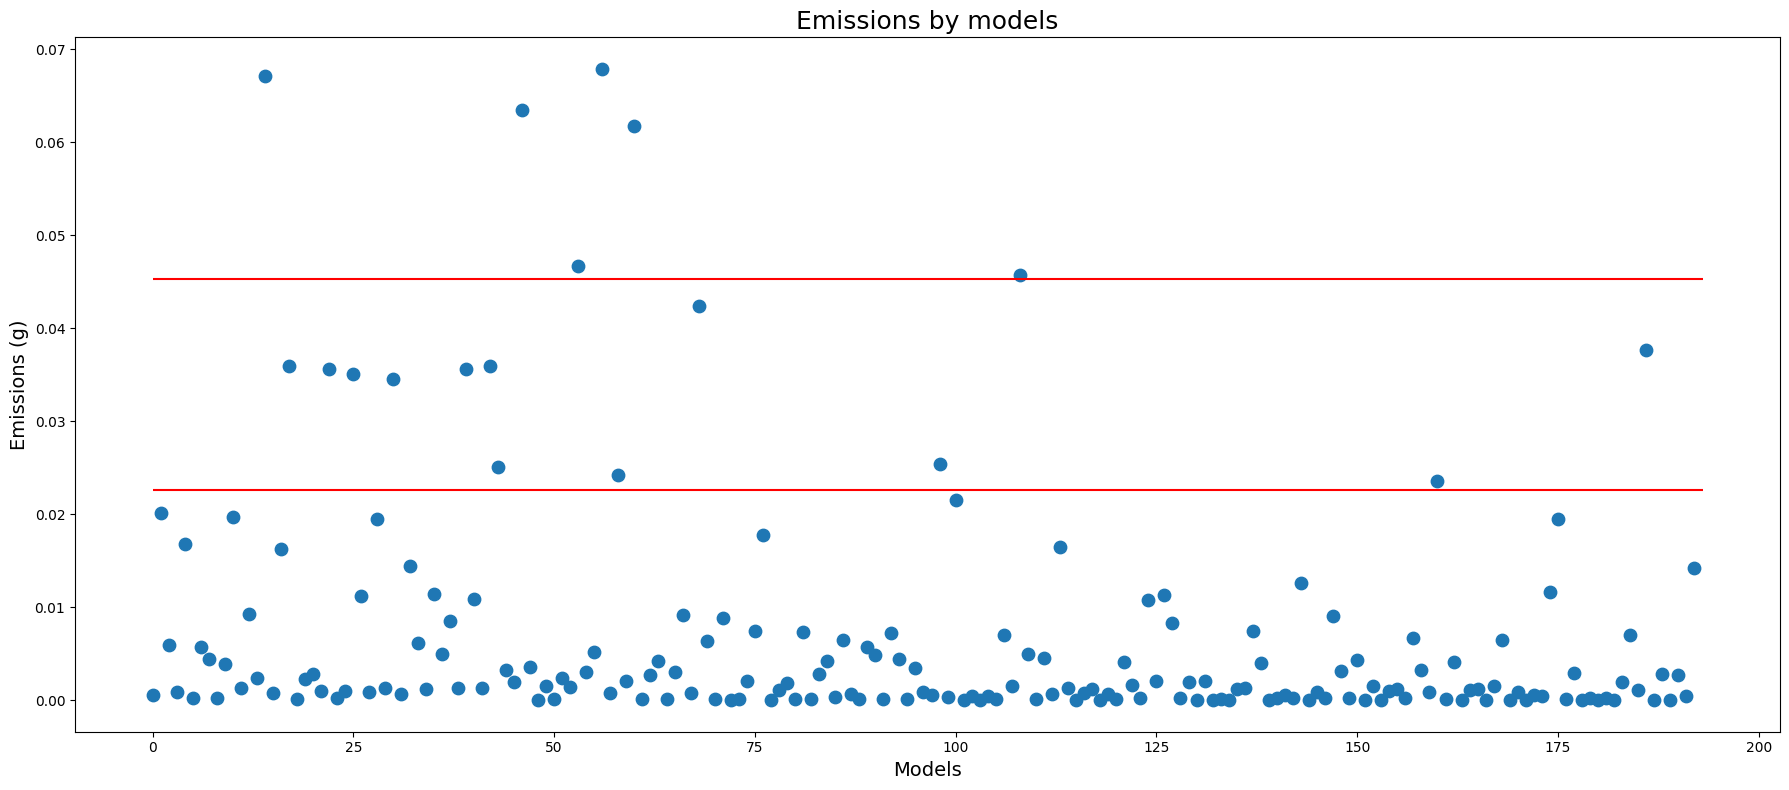
\includegraphics[scale=0.25]{images/situazione-attuale.png}
    \caption{Emissioni prodotte dai vari modelli}
\end{figure}

\noindent L'esperimento è stato condotto su dataset presenti all'interno della libreria python RecBole\footnote{\href{http://recbole.io}{RecBole}}{}, una libreria open-source che offre un'implementazione di modelli di raccomandazione. I dataset utilizzati per l'addestramento dei modelli sono:
\begin{itemize}
    \item \textbf{MovieLens-1M}\footnote{\href{https://github.com/RUCAIBox/RecSysDatasets/blob/master/conversion_tools/usage/MovieLens.md}{Dataset MovieLens}}{}
    \item \textbf{Amazon\_Book\_60core\_kg} \footnote{\href{https://github.com/RUCAIBox/RecSysDatasets/blob/master/conversion_tools/usage/Amazon-book-KG.md}{Dataset Amazon\_Book\_60core\_kg}}{}
    \item \textbf{Mind}\footnote{\href{https://github.com/RUCAIBox/RecSysDatasets/blob/master/conversion_tools/usage/MIND.md}{Dataset MIND}}{}
\end{itemize}




    \newpage
    \section{Dataset del regressore}
In questo capitolo si analizza il dataset utilizzato e come questo è stato trattato per l'addestramento dei modelli. Inoltre, si descrivono le feature di input e output del modello.

\noindent Il dataset nella sua totalità è composto da 13 feature di input e una feature di output. Le feature di input possiamo suddividerle in 4 categorie:
\begin{itemize}
    \item \textbf{Feature relative al dataset}, quali \textit{n\_users}, \textit{n\_items}, \textit{n\_inter}, \textit{sparsity}
    \item \textbf{Feature relative al knowledge graph}, quali \textit{kg\_entities}, \textit{kg\_relations}, \textit{kg\_triples}, \textit{kg\_items}
    \item \textbf{Feature relative all'hardware utilizzato per l'addestramento}, quali \textit{cpu\_cores}, \textit{ram\_size}, \textit{is\_gpu}
    \item \textbf{Feature relative al modello}, quali \textit{model\_name}, \textit{model\_type}
\end{itemize}
Nel dataset sono presenti 201 righe (dunque 201 esperimenti distinti).
\subsection{Descrizione delle feature di output}
La feature di output \textit{emissions} rappresenta le emissioni di CO$_2$eq prodotte dalla macchina durante l'addestramento del modello.
\subsection{Descrizione delle feature di input}
\begin{center}
\begin{table}[H]
    \centering
    \begin{tabularx}{\textwidth}{|c|X|}
        \hline
        \textbf{Feature} & \textbf{Descrizione} \\
        \hline
        n\_users & Numero di utenti presenti nel dataset \\
        \hline
        n\_items & Numero di items presenti nel dataset \\
        \hline
        n\_inter & Numero di interazioni nel dataset. Per interazione si intendono le varie interazioni (valutazioni) tra gli utenti nel dataset e gli item nel dataset \\
        \hline
        sparsity & Sparsità del dataset. La sparsità indica la percentuale di valori mancanti nel dataset (quindi mancanza di interazione tra utenti e item)\\
        \hline
        kg\_entities & Numero di entità nel knowledge graph. Un'entità è un oggetto distintivo o un concetto unico all'interno del Knowledge Graph \\
        \hline
        kg\_relations & Numero di relazioni nel knowledge graph. Le relazioni rappresentano i legami o collegamenti tra le entità all'interno del Knowledge Graph. Sono spesso definite dai predicati nelle triple \\
        \hline
        kg\_triples & Numero di triple nel knowledge graph. Una triple è una struttura dati fondamentale nel Knowledge Graph che consiste in tre parti: soggetto, predicato e oggetto. Queste triple rappresentano le relazioni tra le entità \\
        \hline
        kg\_items & Numero di items nel knowledge graph. Gli "Items" nel contesto del Knowledge Graph sono gli oggetti specifici o le entità che sono inclusi nel grafo \\
        \hline
        cpu\_cores & Numero di core della CPU \\
        \hline
        ram\_size & Dimensione della RAM \\
        \hline
        is\_gpu & Booleano che indica se la macchina ha usato una GPU per l'addestramento \\
        \hline
        model\_name & Nome del modello \\
        \hline
        model\_type & Tipo del modello \\
        \hline
    \end{tabularx}
    \caption{Descrizione delle feature di input}
\end{table}
\end{center}

Per quanto riguarda la feature \textit{model\_type} abbiamo i seguenti valori:
\begin{itemize}
    \item \textbf{General}: Modelli che si basano su tecniche tradizionali
    \item \textbf{Knowledge}: Modelli che incorporano conoscenza esterna (knowledge graph) per migliorare le raccomandazioni
\end{itemize}

Per quanto riguarda la feature \textit{model\_name} abbiamo i seguenti valori:
\begin{itemize}
    \item \textbf{BPR} \cite{BPR}: General
    \item \textbf{CDAE} \cite{CDAE}: General
    \item \textbf{CFKG} \cite{CFKG}: Knowledge
    \item \textbf{CKE} \cite{CKE}: Knowledge
    \item \textbf{DGCF} \cite{DGCF}: Knowledge
    \item \textbf{DMF} \cite{DMF}: General
    \item \textbf{DiffRec} \cite{DiffRec}: General
    \item \textbf{ENMF} \cite{ENMF}: General 
    \item \textbf{FISM} \cite{FISM}: General
    \item \textbf{GCMC} \cite{GCMC}: General
    \item \textbf{ItemKNN} \cite{ItemKNN}: General
    \item \textbf{KGCN} \cite{KGCN}: Knowledge
    \item \textbf{KGIN}: \cite{KGIN} Knowledge
    \item \textbf{KGNNLS} \cite{KGNNLS}: Knowledge
    \item \textbf{KTUP} \cite{KTUP}: Knowledge
    \item \textbf{LDiffRec} \cite{LDiffRec}: General
    \item \textbf{LINE} \cite{LINE}: General
    \item \textbf{LightGCN} \cite{LightGCN}: General
    \item \textbf{MKR} \cite{MKR}: Knowledge
    \item \textbf{MacridVAE} \cite{MacridVAE}: General
    \item \textbf{MultiDAE} \cite{MultiDAE}: General
    \item \textbf{MultiVAE} \cite{MultiVAE}: General
    \item \textbf{NCEPLRec} \cite{NCEPLRec}: General
    \item \textbf{NCL} \cite{NCL}: General
    \item \textbf{NGCF} \cite{NGCF}: General
    \item \textbf{NeuMF} \cite{NeuMF}: General
    \item \textbf{Pop}: General
    \item \textbf{Random}: General
    \item \textbf{RecVAE} \cite{RecVAE}: General
    \item \textbf{RippleNet} \cite{RippleNet}: Knowledge
    \item \textbf{SGL} \cite{SGL}: General
    \item \textbf{SLIMElastic} \cite{SLIMElastic}: General
    \item \textbf{SimpleX} \cite{SimpleX}: General
    \item \textbf{SpectralCF} \cite{SpectralCF}: General
    \item \textbf{EASE} \cite{EASE}: General
    \item \textbf{NAIS} \cite{NAIS}: General
    \item \textbf{ADMMSLIM} \cite{ADMMSLIM}: General
    \item \textbf{ConvNCF} \cite{ConvNCF}: General
    \item \textbf{NNCF} \cite{NNCF}: General
\end{itemize}

Altri valori unici presenti per le varie feature di input sono:
\begin{itemize}
    \item \textbf{n\_users}: [22155, 23679, 6040]
    \item \textbf{n\_items}: [54458, 4414, 3706]
    \item \textbf{n\_inter}: [1465871, 1048575, 1000209]
    \item \textbf{sparsity}: [0.99878504, 0.98996762, 0.95531637]
    \item \textbf{kg\_entities}: [26315, 0, 79347]
    \item \textbf{kg\_relations}: [16, 0, 49]
    \item \textbf{kg\_triples}: [96476, 0, 385923]
    \item \textbf{kg\_items}: [11446, 0, 3655]
    \item \textbf{cpu\_cores}: [12, 4]
    \item \textbf{ram\_size}: [64, 16, 27.40581512]
    \item \textbf{is\_gpu}: [1, 0]
\end{itemize}
\subsection{Pre-Processing}

Per poter sfruttare le feature di input per l'addestramento del modello, è stato necessario effettuare un pre-processing. Le feature \textit{model\_name} e \textit{model\_type} sono state trasformate in variabili numeriche. In particolare il valore \textit{general} è stato trasformato in 0 e il valore \textit{knowledge} è stato trasformato in 1.
Per quanto riguarda la feature \textit{model\_name}, ogni valore è stato trasformato in un numero intero univoco. In questo modo, il modello può sfruttare queste feature per l'addestramento.
Prima di cominciare con l'addestramento dei modelli la feature di output è stata separata dalle feature di input. I dati sono poi stati suddivisi rispettivamente in training set e test set. In particolare il 70\% dei dati è stato usato per l'addestramento, mentre il 30\% è stato usato per la valutazione. Inoltre, mediante il \textit{random\_state}=2, è garantita la riproducibilità dell'esperimento.


    \newpage
    \section{Modelli di regressione}
\subsection{Introduzione ai regressori}
I regressori sono dei modelli di machine learning il cui obiettivo è quello di prevedere un valore numerico continuo (in questo caso il valore delle emissioni).
I regressori vengono valutati sulla base di metriche quali, per esempio, l'errore quadratico medio (MSE), l'errore assoluto medio (MAE), e l'errore quadrato logaritmico medio (MSLE).

\subsection{Regressori utilizzati}
In questo lavoro sono stati utilizzati i seguenti regressori:
\begin{itemize}
    \item \textbf{Support Vector Regression (SVR)}\footnote{\href{https://scikit-learn.org/stable/modules/generated/sklearn.svm.SVR.html}{SVR}}{}
    \item \textbf{Decision Tree Regressor} \footnote{\href{https://scikit-learn.org/stable/modules/generated/sklearn.tree.DecisionTreeRegressor.html}{Decision Tree Regressor}}{}
    \item \textbf{Random Forest Regressor} \footnote{\href{https://scikit-learn.org/stable/modules/generated/sklearn.ensemble.RandomForestRegressor.html}{Random Forest Regressor}}{}
    \item \textbf{AdaBoost Regressor} \footnote{\href{https://scikit-learn.org/stable/modules/generated/sklearn.ensemble.AdaBoostRegressor.html}{AdaBoost Regressor}}{}
\end{itemize}
\subsubsection{Support Vector Regression (SVR)}
%add a footnote to SVM
La SVR è un algoritmo che estende il concetto di Support Vector Machine (SVM)\footnote{Algoritmi di classificazione che cercano di trovare un iperpiano ottimale per ottenere separabilità lineare}{} al caso della regressione.
\begin{figure}[H]
    \centering
    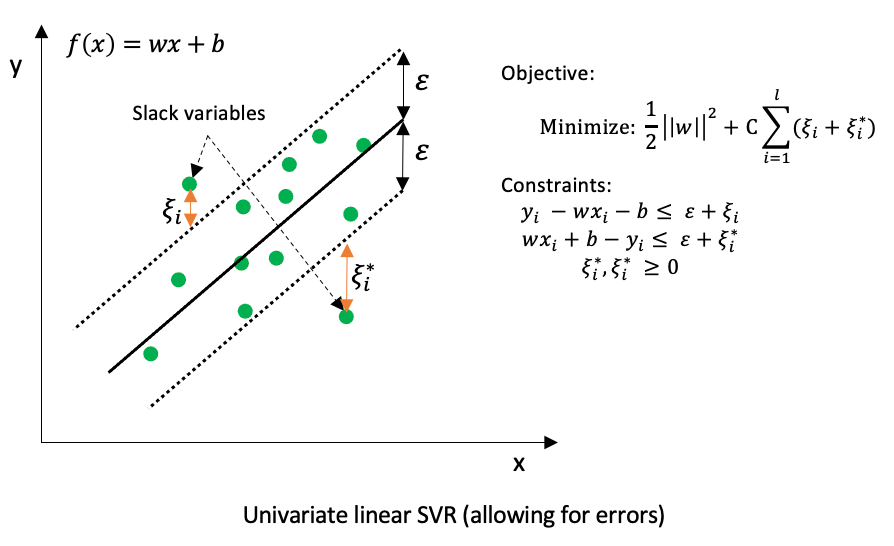
\includegraphics[scale=0.5]{images/SVR.png}
    \caption*{Esempio di SVR}
\end{figure} \newpage
\noindent In questo lavoro il modello è stato costruito usando gli iperparametri di default. Questi ultimi sono:
\begin{itemize}
    \item \textbf{kernel=rbf}: E' il tipo di Kernel\footnote{Funzione matematica usata per mappare i dati originali in uno spazio di dimensione superiore}{} utilizzato. Questo kernel valuta quanto due punti siano simili sulla base della loro distanza
    \item \textbf{degree=3}:  grado del polinomio utilizzato per la trasformazione dei dati nello spazio
    \item \textbf{gamma=scale}: coefficiente del kernel
    \item \textbf{coef0=0.0}: termine indipendente nel kernel
    \item \textbf{tol=0.001}: tolleranza per il criterio di arresto
    \item \textbf{C=1.0}: parametro di regolarizzazione
    \item \textbf{epsilon=0.1}:  controlla la tolleranza del modello nei confronti degli errori nella predizione
    \item \textbf{shrinking=True}: se abilitare o meno la riduzione del set di supporto
    \item \textbf{cache\_size=200}: dimensione della cache in MB
    \item \textbf{max\_iter=-1}: numero massimo di iterazioni. -1 indica nessun limite
\end{itemize}


\subsubsection{Decision Tree Regressor}

I Decision Tree Regressors sono modelli di regressione basati su alberi decisionali. Questi algoritmi suddividono ripetutamente il set di dati in base alle caratteristiche (features) per creare una struttura ad albero che rappresenta la relazione di decisione. Ogni nodo interno dell'albero rappresenta una decisione basata su una caratteristica, e le foglie dell'albero contengono i valori di output previsti.
\begin{figure}[H]
    \centering
    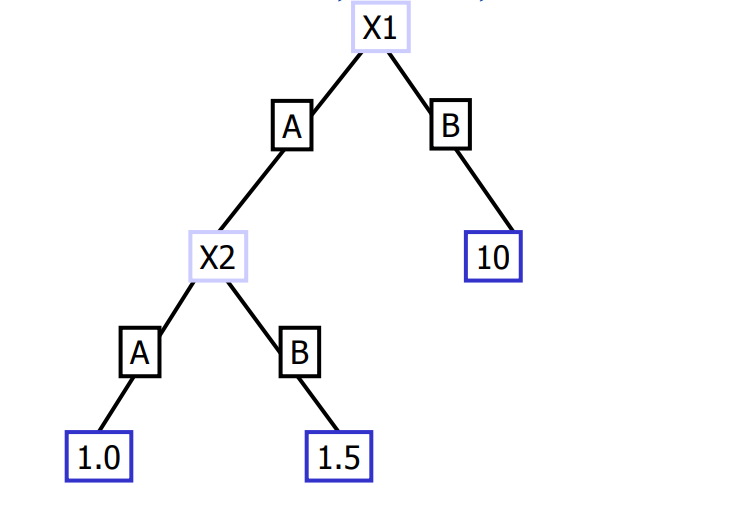
\includegraphics[scale=0.5]{images/DecisionTreeRegressor.png}
    \caption*{Esempio di albero decisionale di regressione}
\end{figure}

\noindent In questo lavoro due iperparametri sono stati decisi all'atto della costruzione del modello:
\begin{itemize}
    \item \textbf{max\_depth=5}: profondità massima dell'albero
    \item \textbf{random\_state=3}:  controlla la casualità nell'addestramento del modello. Quando viene fissato a un numero intero specifico l'addestramento del modello sarà deterministico, cioè produrrà gli stessi risultati in ogni esecuzione
\end{itemize}
\noindent mentre gli altri iperparametri sono stati lasciati ai valori di default:
\begin{itemize}
    \item \textbf{criterion=squared\_error}: Criterio per stabilire la qualità di una suddivisione
    \item \textbf{splitter=best}: Strategia per scegliere la suddivisione in ogni nodo
    \item \textbf{min\_samples\_split=2}: Numero minimo di campioni richiesti per suddividere un nodo interno
    \item \textbf{min\_samples\_leaf=1}: Numero minimo di campioni richiesti per essere in una foglia
    \item \textbf{min\_weight\_fraction\_leaf=0.0}: La frazione minima dei campioni totali (pesati) necessaria affinché si verifichi un nodo foglia
    \item \textbf{max\_features=None}: Numero di features da considerare quando si cerca la migliore suddivisione. None indica tutte
    \item \textbf{max\_leaf\_nodes=None}: Numero massimo di foglie. None indica nessun limite
    \item \textbf{min\_impurity\_decrease=0.0}: Un nodo verrà suddiviso se questa suddivisione induce una diminuzione dell'impurità maggiore o uguale a questo valore
    \item \textbf{ccp\_alpha=0.0}: Parametro di complessità usato per la potatura
    \item \textbf{monotonic\_constraints=None}: Vincoli monotoni sui valori delle features
\end{itemize}

\subsubsection{Random Forest Regressor}
I Random Forest Regressors sono modelli di regressione basati su alberi decisionali. Vengono costruiti su più alberi decisionali che combinano le loro previsioni per ottenere una previsione più accurata e stabile.
\begin{figure}[H]
    \centering
    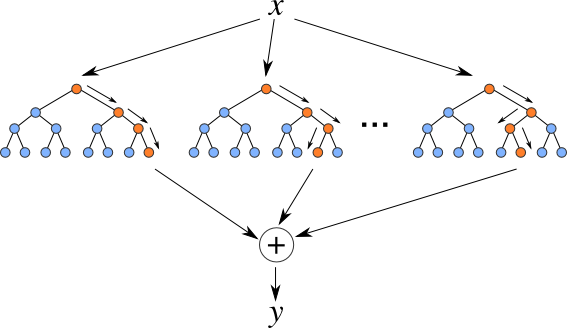
\includegraphics[scale=0.5]{images/RandomForestRegressor.png}
    \caption*{Esempio di Random Forest Regresor}
\end{figure}

\noindent In questo lavoro tre iperparametri sono stati decisi all'atto della costruzione del modello:
\begin{itemize}
    \item \textbf{n\_estimators=500}: numero di alberi nella foresta
    \item \textbf{max\_depth=5}: profondità massima dell'albero
    \item \textbf{random\_state=3}:  controlla la casualità nell'addestramento del modello. Quando viene fissato a un numero intero specifico l'addestramento del modello sarà deterministico, cioè produrrà gli stessi risultati in ogni esecuzione
\end{itemize}

\noindent mentre gli altri iperparametri sono stati lasciati ai valori di default:
\begin{itemize}
    \item \textbf{criterion=squared\_error}: Criterio per stabilire la qualità di una suddivisione
    \item \textbf{min\_samples\_split=2}: Numero minimo di campioni richiesti per suddividere un nodo interno
    \item \textbf{min\_samples\_leaf=1}: Numero minimo di campioni richiesti per essere in una foglia
    \item \textbf{min\_weight\_fraction\_leaf=0.0}: La frazione minima dei campioni totali (pesati) necessaria affinché si verifichi un nodo foglia
    \item \textbf{max\_features=1}: Numero di features da considerare quando si cerca la migliore suddivisione
    \item \textbf{max\_leaf\_nodes=None}: Numero massimo di foglie. None indica nessun limite
    \item \textbf{min\_impurity\_decrease=0.0}: Un nodo verrà suddiviso se questa suddivisione induce una diminuzione dell'impurità maggiore o uguale a questo valore
    \item \textbf{ccp\_alpha=0.0}: Parametro di complessità usato per la potatura
    \item \textbf{bootstrap=True}: Se utilizzare il bootstrap per la costruzione degli alberi
    \item \textbf{oob\_score=False}: Se calcolare l'errore out-of-bag
    \item \textbf{n\_jobs=None}: Numero di lavori da eseguire in parallelo. None indica 1
    \item \textbf{warm\_start=False}: Se utilizzare la soluzione precedente come inizializzazione
    \item \textbf{max\_samples=None}: Numero massimo di campioni da utilizzare per la costruzione di ciascun albero. None indica tutti
    \item \textbf{monotonic\_constraints=None}: Vincoli monotoni sui valori delle features
\end{itemize}
\newpage
\subsubsection{AdaBoost Regressor}
L'AdaBoost Regressor è un modello basato sull'algoritmo di boosting AdaBoost\footnote{Crea un modello forte combinando modelli più deboli, ognuno allenato su diverse parti del dataset}{}. Questo algoritmo costruisce un modello di previsione combinando più modelli di previsione più deboli.
\begin{figure}[H]
    \centering
    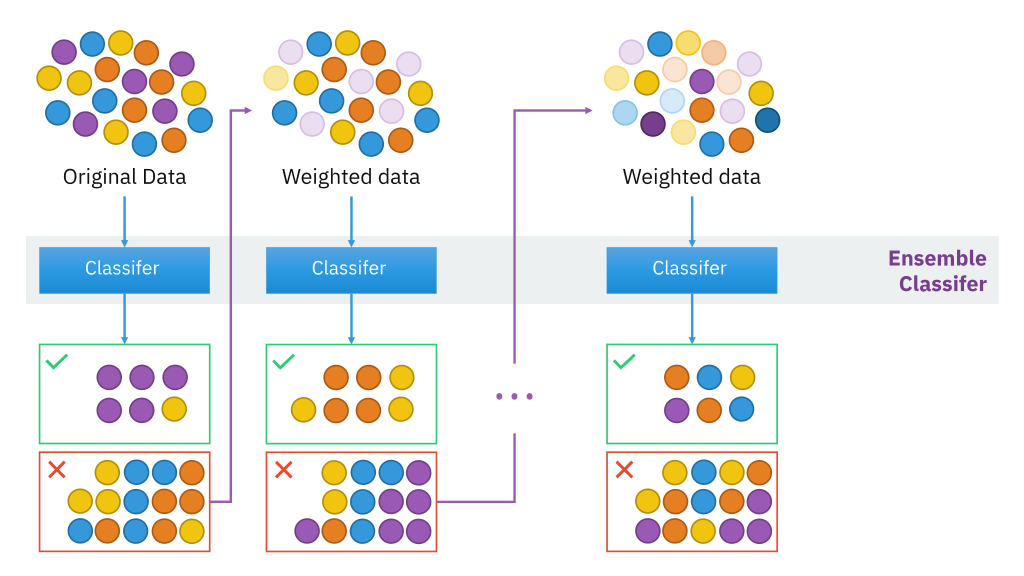
\includegraphics[scale=0.4]{images/AdaBoost.png}
    \caption*{Struttura di modello basato su AdaBoost}
\end{figure}

\noindent In questo lavoro due iperparametri sono stati decisi all'atto della costruzione del modello:

\begin{itemize}
    \item \textbf{n\_estimators=500}: numero di stimatori
    \item \textbf{random\_state=3}:  controlla la casualità nell'addestramento del modello. Quando viene fissato a un numero intero specifico l'addestramento del modello sarà deterministico, cioè produrrà gli stessi risultati in ogni esecuzione
\end{itemize}

\noindent mentre gli altri iperparametri sono stati lasciati ai valori di default:
\begin{itemize}
    \item \textbf{estimator=None}: stimatore base. Se None, viene utilizzato DecisionTreeRegressor
    \item \textbf{learning\_rate=1.0}: tasso di apprendimento
    \item \textbf{loss=linear}: funzione di perdita
\end{itemize}


    \newpage
    \section{Risultati}

In questo capitolo si analizzano i risultati degli esperimenti che sono stati condotti. I regressori utilizzati sono stati valutati utilizzando le seguenti metriche per la regressione:
\begin{itemize}
    %add the mathematic formula of each error
    \item \textbf{Mean Absolute Error (MAE)}: è la media della differenza assoluta tra le previsioni e i valori reali.
    \begin{equation*}
        MAE = \frac{1}{n} \sum_{i=1}^{n} |y_i - \hat{y}_i|
    \end{equation*}
    \item \textbf{Root Mean Squared Error (RMSE)}: è la radice quadrata della media della differenza tra le previsioni e i valori reali al quadrato.
    \begin{equation*}
        RMSE = \sqrt{\frac{1}{n} \sum_{i=1}^{n} (y_i - \hat{y}_i)^2}
    \end{equation*}
    \item \textbf{Mean Logarithmic Squared Error (MSLE)}: è la media del logaritmo dei quadrati degli errori.
    \begin{equation*}
        MSLE = \frac{1}{n} \sum_{i=1}^{n} (\log(y_i + 1) - \log(\hat{y}_i + 1))^2
    \end{equation*}
\end{itemize}

\subsection{Risultati ottenuti}

\begin{table}[H]
    \centering
    \begin{tabular}{|>{\centering\arraybackslash}m{5cm}|c|c|c|c|}
        \hline
        \textbf{Regressor} & \textbf{MAE} & \textbf{RMSE} & \textbf{MSLE} \\ [10pt]
        \hline
        SVR & 0.0288215 & 0.0008862 & 0.0008537 \\ [10pt]
        \hline
        Decision Tree & 0.0048531 & 0.0000969 & 0.0000918 \\ [10pt]
        \hline
        Random Forest & 0.0054369 & 0.0001088 & 0.0001026 \\ [10pt]
        \hline
        AdaBoost & 0.0071778 & 0.0001113 & 0.0001059 \\ [10pt]
        \hline
    \end{tabular}
    \caption{Risultati ottenuti}
    \label{tab:results}
\end{table}

\begin{table}[H]
    \centering
    \begin{tabular}{c c}
        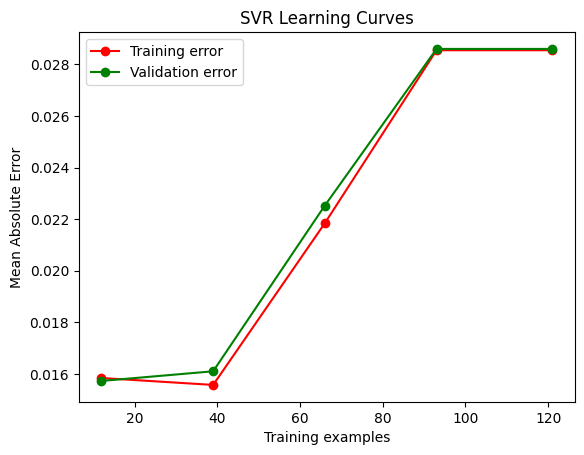
\includegraphics[scale=0.3]{images/SVR_lc.png} & 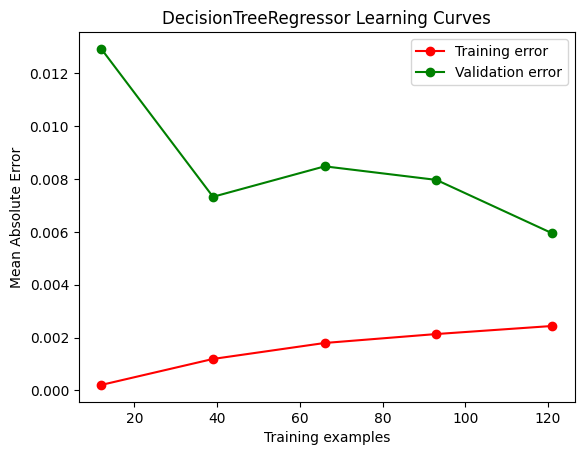
\includegraphics[scale=0.3]{images/DecisionTree_lc.png} \\
        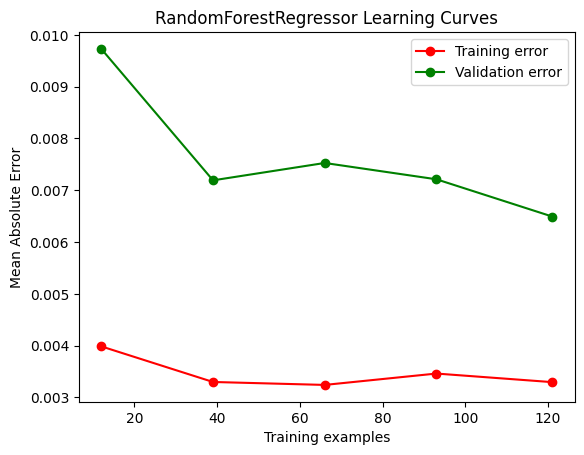
\includegraphics[scale=0.3]{images/RandomForestRegressor_lc.png} & 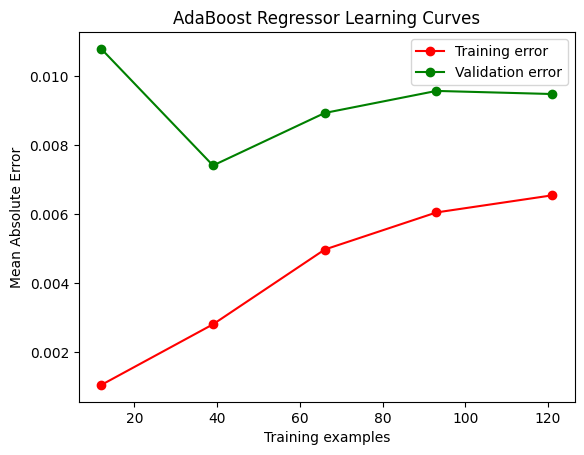
\includegraphics[scale=0.3]{images/AdaBoostRegressor_lc.png} \\
    \end{tabular}
    \caption{Learning curve dei regressori}
    \label{tab:lc}
\end{table}

\subsection{Analisi dei risultati}


    \paragraph{\textbf{SVR}.}
    Dal punto di vista delle metriche il regressore SVR ha ottenuto i peggiori risultati in termini di MAE, RMSE e MSLE. La learning curve mostra che il modello è in overfitting, infatti gli errori aumentano all'aumentare del numero di istanze.
   
   
    \paragraph{\textbf{Decision Tree Regressor}.}
    Dal punto di vista delle metriche, il Decision Tree Regressor ha ottenuto i migliori risultati. 
    La learning curve mostra una curva di training che aumenta all'aumentare del numero di istanze, mentre la curva di validation diminuisce. Le due curve si avvicinano, ma non si sovrappongono. Sembra esserci un leggero underfitting.
    \paragraph{\textbf{Random Forest Regressor}.}
    Dal punto di vista delle metriche il Random Forest Regressor risulta essere il secondo miglior modello.
    La learning curves di train e di validation set diminuiscono entrambe all'aumentare del numero di istanze, ma non si sovrappongono. Anche qui sembra esserci underfitting.
    \paragraph{\textbf{AdaBoost Regressor}.}
    Dal punto di vista delle metriche il AdaBoost Regressor ha ottenuto risultati peggiori rispetto al Random Forest Regressor ma migliori rispetto al SVR.
    La learning curve mostrano che il modello non è riuscito a generalizzare bene


\subsection{Conclusioni}
Il dataset sembra essere troppo piccolo per poter generalizzare bene i modelli. Inoltre, il dataset è molto sbilanciato, con pochi valori per ogni feature. Questo potrebbe essere un motivo per cui i modelli non generalizzano bene. Inoltre, i modelli non sono stati ottimizzati, quindi potrebbero essere migliorati mediante ricerca di iperparametri.
Per i risultati attuali, il Decision Tree Regressor è il modello migliore.
    \newpage
    \bibliography{bibliography}
\end{document}
